\hypertarget{twoplates_8h}{
\section{src/twoplates.h File Reference}
\label{twoplates_8h}\index{src/twoplates.h@{src/twoplates.h}}
}
Two symmetrical plates geometry. 

{\tt \#include $<$geometry.h$>$}\par


Include dependency graph for twoplates.h:\nopagebreak
\begin{figure}[H]
\begin{center}
\leavevmode
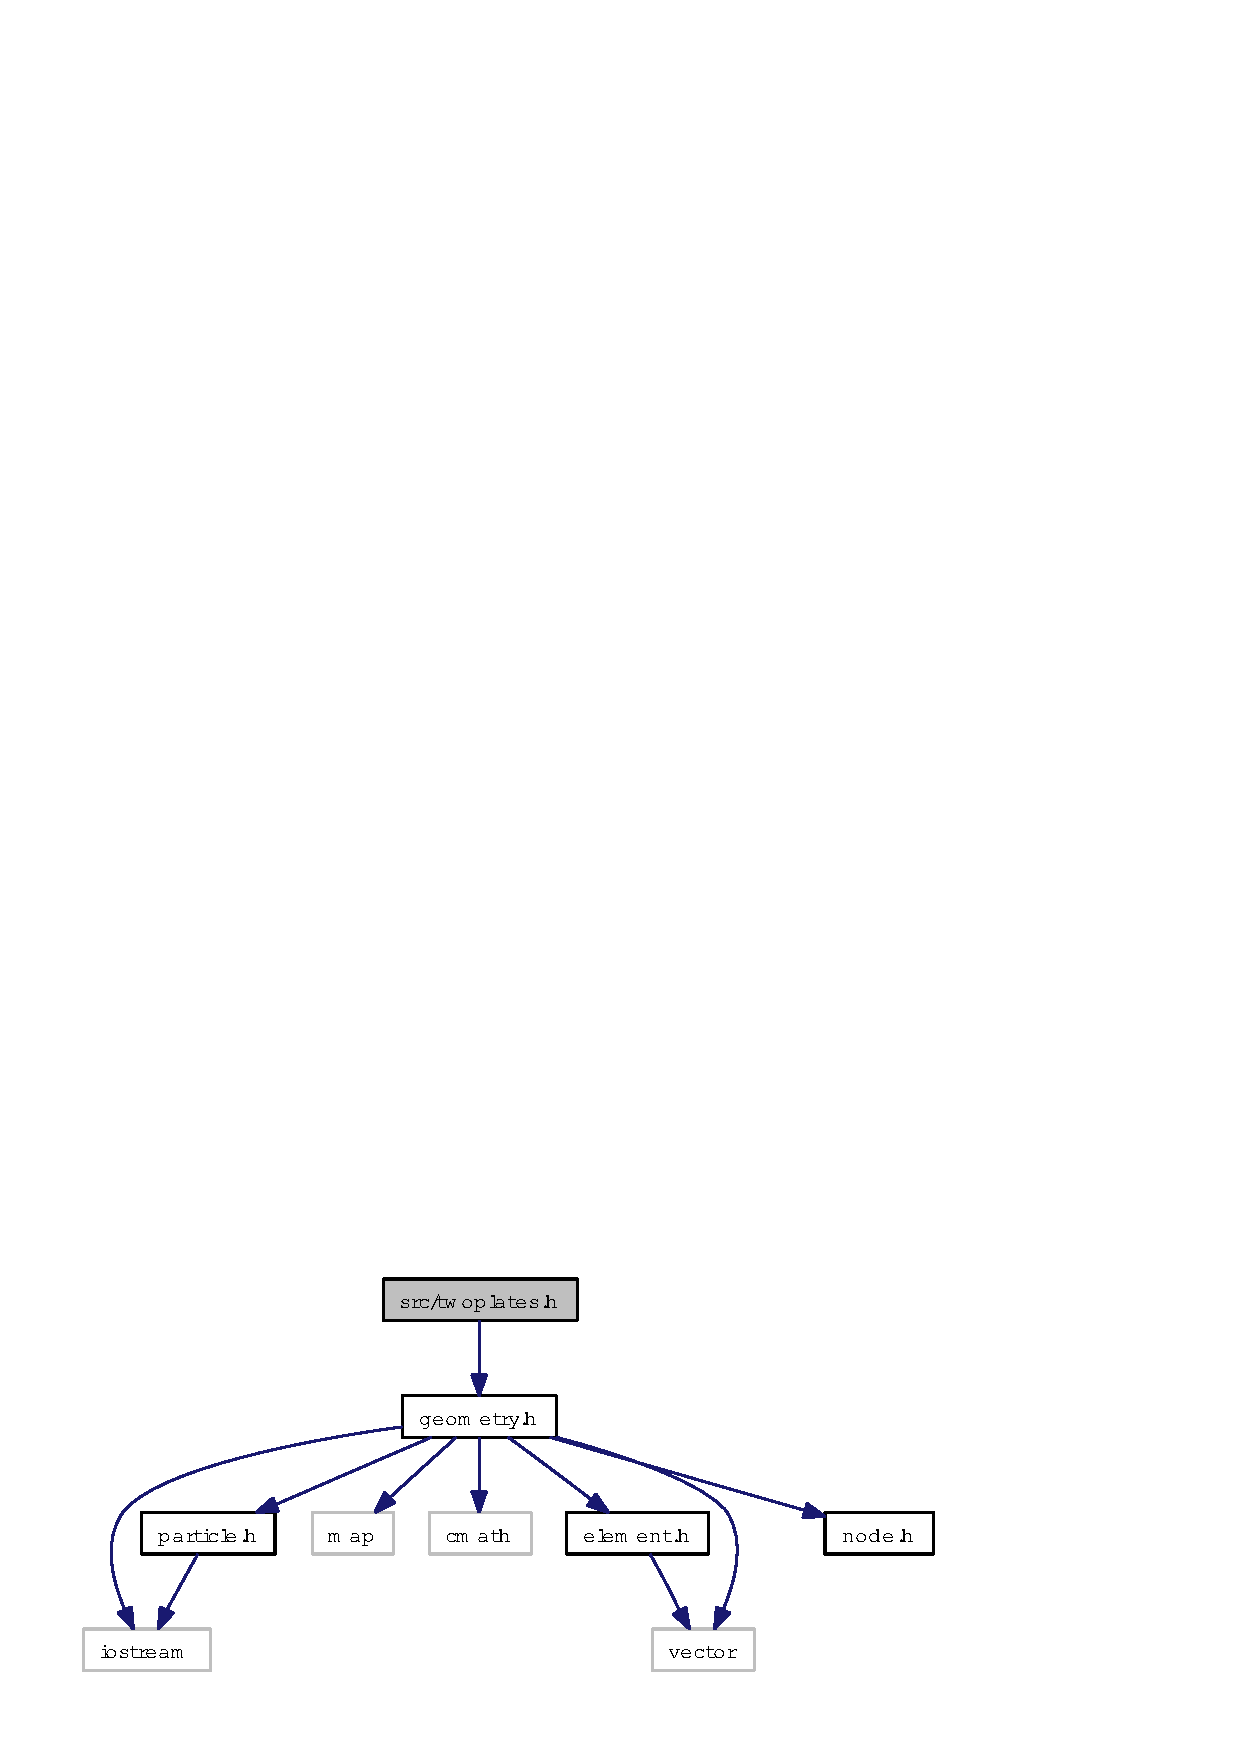
\includegraphics[width=226pt]{twoplates_8h__incl}
\end{center}
\end{figure}


This graph shows which files directly or indirectly include this file:\nopagebreak
\begin{figure}[H]
\begin{center}
\leavevmode
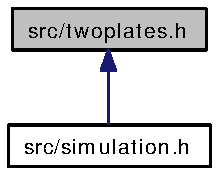
\includegraphics[width=70pt]{twoplates_8h__dep__incl}
\end{center}
\end{figure}
\subsection*{Classes}
\begin{CompactItemize}
\item 
class \hyperlink{classTwoPlates}{TwoPlates}
\end{CompactItemize}


\subsection{Detailed Description}
Two symmetrical plates geometry. 

\hyperlink{classGeometry}{Geometry} with origin in s=0 defined by s-length and initial plate separation (constant slope).

\begin{Desc}
\item[Author:]Daniel Iglesias $<$\href{mailto:daniel.iglesias@ciemat.es}{\tt daniel.iglesias@ciemat.es}$>$ \end{Desc}
